% PRL look and style (easy on the eyes)
\documentclass[aps,pre,twocolumn,nofootinbib,superscriptaddress,linenumbers]{revtex4-1}
% Two-column style (for submission/review/editing)
%\documentclass[aps,prl,preprint,nofootinbib,superscriptaddress,linenumbers]{revtex4-1}

\pdfoutput=1
\usepackage[pdftex]{graphicx}

\usepackage{alltt}

%\usepackage{palatino}

%\usepackage{palatino}
% Change to a sans serif font.
\usepackage{sourcesanspro}
\renewcommand*\familydefault{\sfdefault} %% Only if the base font of the document is to be sans serif
\usepackage[T1]{fontenc}
%\usepackage[font=sf,justification=justified]{caption}
\usepackage[font=sf]{floatrow}

% Rework captions to use sans serif font.
\makeatletter
\renewcommand\@make@capt@title[2]{%
 \@ifx@empty\float@link{\@firstofone}{\expandafter\href\expandafter{\float@link}}%
  {\sf\textbf{#1}}\sf\@caption@fignum@sep#2\quad
}%
\makeatother

\usepackage{listings} % For code examples
\usepackage[usenames,dvipsnames,svgnames,table]{xcolor}

\usepackage{amsmath}
\usepackage{amssymb}
%\usepackage[mathbf,mathcal]{euler}
%\usepackage{citesort}
\usepackage[caption=false]{subfig}
\usepackage{dcolumn}
\usepackage{boxedminipage}
\usepackage{verbatim}
\usepackage[colorlinks=true,citecolor=blue,linkcolor=blue]{hyperref}
\usepackage[group-separator={,}]{siunitx}

% Justification
\captionsetup{singlelinecheck=off}

% Pretty-printing of shell commands
\newcommand{\shellcmd}[1]{\\\ \texttt{\scriptsize\# #1}\\}

% The figures are in a figures/ subdirectory.
\graphicspath{{../figures/}}


% \newcommand{\pyitc}{\url{http://www.simtk.org/home/bayesian-itc}} % URL of pyITC project homepage

%% DOCUMENT %%%%%%%%%%%%%%%%%%%%%%%%%%%%%%%%%%%%%%%%%%%%%%%%%%%%%%%%%%%%%%%%%%%%
\begin{document}

%% TITLE %%%%%%%%%%%%%%%%%%%%%%%%%%%%%%%%%%%%%%%%%%%%%%%%%%%%%%%%%%%%%%%%%%%%
\title{Ensembler: Enabling high-throughput molecular simulations at the superfamily scale}

\author{Daniel L. Parton}
  \affiliation{Computational Biology Program, Sloan Kettering Institute, Memorial Sloan Kettering Cancer Center, New York, NY 10065}
  %\email{daniel.parton@choderalab.org}
\author{Patrick B. Grinaway}
  \affiliation{Computational Biology Program, Sloan Kettering Institute, Memorial Sloan Kettering Cancer Center, New York, NY 10065}
  %\email{patrick.grinaway@choderalab.org}
\author{John D. Chodera}
 \thanks{Corresponding author}
 \email{john.chodera@choderalab.org}
  \affiliation{Computational Biology Program, Sloan Kettering Institute, Memorial Sloan Kettering Cancer Center, New York, NY 10065}

\date{\today}

%%%%%%%%%%%%%%%%%%%%%%%%%%%%%%%%%%%%%%%%%%%%%%%%%%%%%%%%%%%%%%%%%%%%%%%%%%%%%%%%%%%%%%%%%%%%%%%%%%%%%%
% ABSTRACT/pacs
%%%%%%%%%%%%%%%%%%%%%%%%%%%%%%%%%%%%%%%%%%%%%%%%%%%%%%%%%%%%%%%%%%%%%%%%%%%%%%%%%%%%%%%%%%%%%%%%%%%%%%
\begin{abstract}

The rapidly expanding body of available genomic and protein structural data provides a rich resource for understanding protein dynamics with biomolecular simulation. 
While computational infrastructure has grown rapidly, simulations on an \emph{omics} scale are not yet widespread, primarily because software infrastructure to enable simulations at this scale have not kept pace. 
It should now be possible to study protein dynamics across entire (super)families, exploiting both available structural biology data and conformational similarities across homologous proteins.
Here, we present a new tool for enabling high-throughput simulation in the genomics era.
{\bf Ensembler} takes any set of sequences---from a single sequence to an entire superfamily---and shepherds them through various stages of modeling and refinement to produce simulation-ready structures.
This includes comparative modeling to all relevant PDB structures (which may span multiple conformational states of interest), reconstruction of missing loops, addition of missing atoms, culling of nearly identical structures, assignment of appropriate protonation states, solvation in explicit solvent, and refinement and filtering with molecular simulation to ensure stable simulation. 
The output of this pipeline is an ensemble of structures ready for subsequent molecular simulations using computer clusters, supercomputers, or distributed computing projects like Folding@home.
{\bf Ensembler} thus automates much of the time-consuming process of preparing protein models suitable for simulation, while allowing scalability up to entire superfamilies.  {\color{red}[JDC: Prior sentence is redundant?]}
A particular advantage of this approach can be found in the construction of kinetic models of conformational dynamics---such as Markov state models---which benefit from a diverse array of initial configurations that span the accessible conformational states to aid sampling.
We demonstrate the power of this approach by constructing models for all catalytic domains in the human tyrosine kinase family, using all available kinase catalytic domain structures from any organism as structural templates.

{\bf Ensembler} is free and open source software licensed under the GNU General Public License (GPL) v2. 
It should run on all major operating systems, and has been tested on Linux and OS X.
The latest release can be installed via the {\tt conda} package manager, and the latest source can be downloaded from \url{https://github.com/choderalab/ensembler}.

\emph{Keywords: molecular dynamics simulation; comparative modeling; distributed simulation}

% TODO expand to all human protein kinases?

\end{abstract}

\maketitle

%%%%%%%%%%%%%%%%%%%%%%%%%%%%%%%%%%%%%%%%%%%%%%%%%%%%%%%%%%%%%%%%%%%%%%%%%%%%%%%%%%%%%%%%%%%%%%%%%%%%%%
% INTRODUCTION
%%%%%%%%%%%%%%%%%%%%%%%%%%%%%%%%%%%%%%%%%%%%%%%%%%%%%%%%%%%%%%%%%%%%%%%%%%%%%%%%%%%%%%%%%%%%%%%%%%%%%%
\section{Introduction}
\label{section:introduction}

Recent advances in genomics and structural biology have helped generate an enormous wealth of protein data at the level of amino-acid sequence and three-dimensional structure.
However, proteins typically exist as an ensemble of thermally accessible conformational states, and static structures provide only a snapshot of their rich dynamical behavior.
Many functional properties---such as the ability to bind small molecules or interact with signaling partners---require transitions between states, encompassing anything from reorganization of sidechains at binding interfaces to domain motions to large scale folding-unfolding events.
Drug discovery could also benefit from a more extensive consideration of protein dynamics, whereby small molecules might be selected based on their predicted ability to bind and trap a protein target in an inactive state~\cite{craik:2009:science:trapping-moving-targets}.

Molecular dynamics (MD) simulations have the capability, in principle, to describe the time evolution of a protein in atomistic detail, and have proven themselves to be a useful tool in the study of protein dynamics.
A number of mature software packages and forcefields are available, and much recent progress has been driven by advances in computing architecture.
For example, many MD packages are now able to exploit GPUs, which provide greatly improved simulation efficiency per unit cost relative to CPUs, while distributed computing platforms such as Folding@home [CITE], GPUGrid [CITE], and Copernicus [CITE] allow scalability on an unprecedented level.
In parallel, methods for building human-understandable models of protein dynamics from noisy simulation data, such as Markov state modeling (MSM) approaches, are now reaching maturity [CITE MSM reviews].
MSM methods in particular have the advantage of being able to aggregate data from multiple independent MD trajectories, facilitating parallelization of production simulations and thus greatly alleviating overall computational cost.
There also exist a number of mature software packages for comparative modeling of protein structures, in which a target protein sequence is modeled using one or more structures as templates [CITE Modeller and Rosetta and a recent homology modeling review].

However, it remains difficult for researchers to exploit the full variety of available protein sequence and structural data in simulation studies, largely due to limitations in software architecture.
For example, the set up of a biomolecular simulation is typically performed manually, encompassing a series of fairly standard (yet time-consuming) steps such as the choice of protein sequence construct and starting structure, addition of missing residues and atoms, solvation with explicit water and salt buffer, choice of simulation parameters, and system relaxation with energy minimization and one or more short MD simulations.
For this reason, simulation studies typically consider only one or a few proteins and starting configurations.

The ability to fully exploit the large base of available protein sequence and structural data in biomolecular simulation studies could open up many interesting avenues for research, enabling the study of entire protein families or superfamilies across multiple organisms.
The similarity between members of a given protein family could be exploited to generate arrays of conformational models, which could be used as starting configurations to aid sampling in MD simulations.
This approach would be highly beneficial for many MD methods, such as MSM construction, which require global coverage of the conformational landscape to realize their full potential, and would also be particularly useful in cases where structural data is present for only a subset of the members of a protein family.
It would also aid in studying protein families known to have multiple metastable conformations---such as kinases---for which the combined body of structural data for the family may cover a large range of these conformations, while the available structures for any individual member might encompass only one or two distinct conformations.

Here, we present the first steps toward bridging the gap between biomolecular simulation software and \emph{omics}-scale sequence and structural data: a fully automated open source framework for building simulation-ready protein models in multiple conformational substates scalable from single sequences to entire superfamilies.
{\bf Ensembler} provides functions for selecting target sequences and homologous template structures, and (by interfacing with a number of external packages) performs pairwise alignments, comparative modeling of target-template pairs, and several stages of model refinement.
As an example application, we have constructed models for the entire set of human tyrosine kinase catalytic domains, using all available structures of protein kinase domains (from any species) as templates.
This results in a total of almost 400,000 models, and we demonstrate that these provide wide-ranging coverage of known functionally relevant conformations.
By using these models as starting configurations for highly parallel MD simulations, we expect their structural diversity to greatly aid in sampling of conformational space.
We anticipate that the tool will prove to be useful in a number of other ways.
For example, the generated models could represent valuable data sets even without subsequent production simulation, allowing exploration of the conformational diversity present within the available structural data for a given protein family.
Furthermore, the automation of simulation set up provides an excellent opportunity to make concrete certain "best practices", such as the choice of simulation parameters.

%%%%%%%%%%%%%%%%%%%%%%%%%%%%%%%%%%%%%%%%%%%%%%%%%%%%%%%%%%%%%%%%%%%%%%%%%%%%%%%%%%%%%%%%%%%%%%%%%%%%%
% DESIGN AND IMPLEMENTATION
%%%%%%%%%%%%%%%%%%%%%%%%%%%%%%%%%%%%%%%%%%%%%%%%%%%%%%%%%%%%%%%%%%%%%%%%%%%%%%%%%%%%%%%%%%%%%%%%%%%%%
\section{Design and Implementation}

{\bf Ensembler} is written in Python, and can be used via a command-line tool ({\tt ensembler}) or via a flexible Python API.

The {\bf Ensembler} modeling pipeline comprises a series of stages which are performed in a defined order. 
A visual overview of the pipeline is shown in Fig.~\ref{figpipeline}.
The various stages of this pipeline are described in detail below.

{\color{red}[JDC: We could really help the reader if we preface each section here with a bit of an introduction of what we're trying to accomplish in each stage.  Otherwise, I worry that each section is a long list of things we do without reference to an overall concept of what the stage is trying to accomplish or why certain decisions were made.]}
{\color{blue}[DLP: Good point. I've added in brief introductions for each section.]}
{\color{red}[JDC: Can you do a bit more here? I feel that the reader may need more orientation.  You've essentially just added a sentence or two at the beginning of each stage that doesn't really enlighten the user as to your terminology (\emph{tempalte} and \emph{target}), your motivation for \emph{why} things are done each stage, or \emph{how} the user is to select among the various options available.]}

\begin{figure*}[tb]
    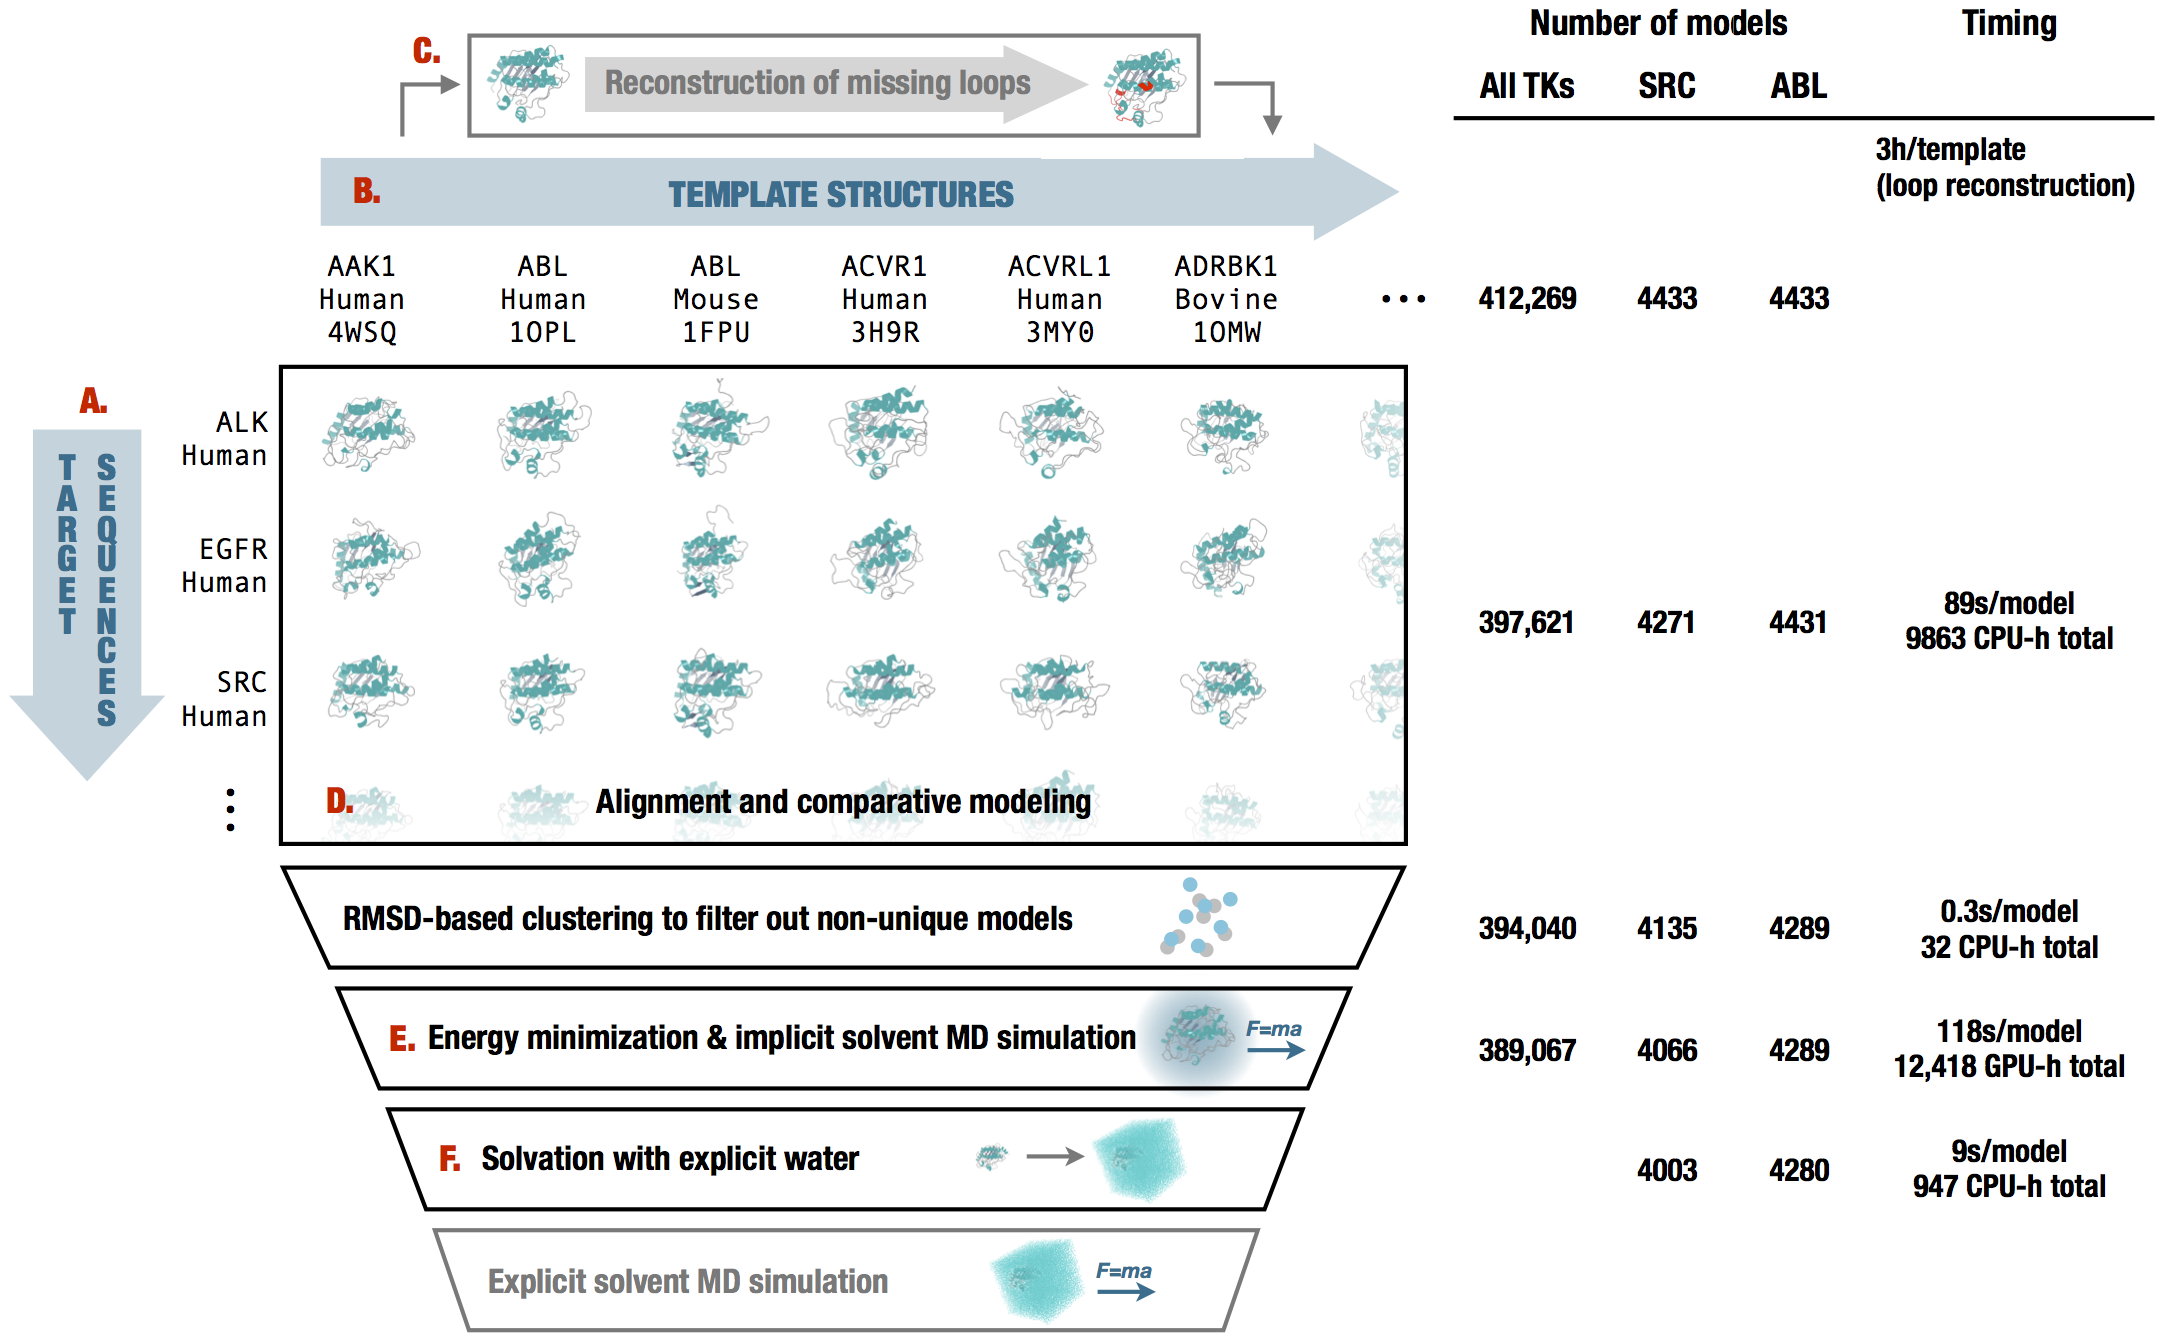
\includegraphics[width=1.0\textwidth]{pipeline/pipeline2}

  \caption{{\bf Diagrammatic representation of the various stages of the Ensembler pipeline.}
  The number of viable models surviving each stage of the pipeline are shown, either for all tyrosine kinases (\emph{All TKs}) or representative individual kinases (\emph{SRC} and \emph{ABL}).
  In addition, the typical timing on a cluster (containing Intel Xeon E5-2665 2.4GHz hyperthreaded processors and NVIDIA GTX-680 or GTX-Titan GPUs) is reported to exemplify the resources required per model and for modeling the entire set of tyrosine kinases.
  Note that \emph{CPU-h} denotes the number of hours consumed by the equivalent of a single hyperthread---parallel execution can reduce wall clock time nearly linearly.
  }
  \label{figpipeline}
\end{figure*}

\subsubsection*{Target selection}

The first stage entails the selection of a set of target protein sequences, i.e. the sequences the user is interested in modeling.
{\color{red}[JDC: Maybe explain what is meant by ``target protein sequences''?  These are the sequences the user is interested in modeling.]}
{\color{blue}[DLP: Addressed.]}

These targets can be defined manually, simply by providing a FASTA-formatted text file containing the desired target sequences with arbitrary identifiers.
The {\tt ensembler} command-line tool also allows targets to be selected from UniProt---a freely accessible resource for protein sequence and functional data (\href{http://www.uniprot.org/}{uniprot.org}) {\color{red}[JDC: Isn't there a real citation for UniProt?]}, using the subcommand {\tt gather\_targets}.
The user specifies a query string with the {\tt -{}-query} flag, which conforms to the same syntax as the search function available on the UniProt website.
For example, {\tt -{}-query `mnemonic:SRC\_HUMAN'} would select the full-length human Src sequence, while {\tt -{}-query `domain:"Protein kinase" AND taxonomy:9606 AND reviewed:yes'} would select all human protein kinases which have been reviewed by a human curator.
In this way, the user may select a single protein, many proteins, or an entire superfamily.
The program outputs a FASTA file, setting the UniProt mnemonic (e.g. {\tt SRC\_HUMAN}) as the identifier for each target protein.

In many cases, it will be desirable to build models of an isolated protein domain, rather than the full-length protein.
The {\tt gather\_targets} subcommand allows protein domains to be selected from UniProt data by passing a regular expression string to the {\tt -{}-domains} flag. 
For example, the above {\tt -{}-query} flag for selecting all human protein kinases returns UniProt entries with domain annotations including "Protein kinase", "Protein kinase 1", "Protein kinase 2", "Protein kinase; truncated", "Protein kinase; inactive", "SH2", "SH3", etc.
To select only domains of the first three types, the following regular expression could be used: {\tt`\^{}Protein kinase(?!; truncated)(?!; inactive)'}.
In this case, target identifiers are set with the form {\tt [UniProt mnemonic]\_D[domain index]}, where the latter part represents a 0-based index for the domain---necessary because a single target protein may contain multiple domains of interest.
Example identifiers: {\tt JAK1\_HUMAN\_D0}, {\tt JAK1\_HUMAN\_D1}.
{\color{red}[JDC: Does it make sense to set some of these coded examples off on their own lines?]}

\subsubsection*{Template selection}

{\bf Ensembler} uses comparative modeling to build models, and as such requires a set of structures to be used as templates.
The second stage thus entails the selection of templates and storage of associated sequences, structures, and identifiers.
These templates can be specified manually, or using the {\tt ensembler gather\_templates} subcommand to automatically select templates from the Protein Data Bank (PDB) or from UniProt.
A recommended approach is to select templates from UniProt which belong to the same protein family as the targets, guaranteeing some degree of homology between targets and templates.
{\color{red}[JDC: Again, can you provide more information about \emph{why} this is being done? What the motivation is, and how the user might expect to select these?]}
{\color{blue}[DLP: Addressed]}

Manual selection of templates simply requires storing the sequences and identifiers in a FASTA file, and the structures as PDB-format coordinate files with filenames matching the identifiers in the sequence file.
The structure residues must also match those in the sequence file.

The {\tt ensembler gather\_templates} subcommand provides methods for selecting template structures from either UniProt or the PDB (\href{http://www.rcsb.org/pdb}), specified by the {\tt -{}-gather\_from} flag.
Both methods select templates at the level of PDB chains---a PDB structure containing multiple chains with identical sequence spans (e.g. for crystal unit cells with multiple asymmetric units) would thus give rise to multiple template structures.

Selection of templates from the PDB simply requires passing a list of PDB IDs as a comma-separated string, e.g. {\tt -{}-query 2H8H,1Y57}.
Specific PDB chain IDs can optionally also be selected via the {\tt -{}-chainids} flag.
The program retrieves structures from the PDB server, as well as associated data from the SIFTS service (\href{http://www.ebi.ac.uk/pdbe/docs/sifts/}{www.ebi.ac.uk/pdbe/docs/sifts}) (CITE: Velankar Nucleic Acids Res 2013), which provides residue-level mappings between PDB and UniProt entries.
The SIFTS data is used to extract template sequences, retaining only residues which are resolved and match the equivalent residue in the UniProt sequence---non-wildtype residues are thus removed from the template structures.
Furthermore, PDB chains with less than a given percentage of resolved residues (default: 70\%) are filtered out.
Sequences are stored in a FASTA file, with identifiers of the form {\tt [UniProt mnemonic]\_D[UniProt domain index]\_[PDB ID]\_[PDB chain ID]}, e.g. {\tt SRC\_HUMAN\_D0\_2H8H\_A}.
Matching residues then extracted from the original coordinate files and stored as PDB-format coordinate files.

Selection of templates from UniProt proceeds in a similar fashion as for target selection; the {\tt -{}-query} flag is used to select full-length proteins from UniProt, while the optional {\tt -{}-domains} flag allows selection of individual domains with a regular expression string.
The returned UniProt data for each protein includes a list of associated PDB chains and their residue spans, and this information is used to select template structures, using the same method as for template selection from the PDB.
If the {\tt -{}-domains} flag is used, then templates are truncated at the start and end of the domain sequence.

Unresolved template residues can optionally be remodeled with the {\tt loopmodel} subcommand, which employs a kinematic closure algorithm {\color{red}[CITE]} provided via the {\tt loopmodel} tool of the Rosetta software suite (CITE: Rosetta and/or loopmodel).
Because fewer loops need to be built during the subsequent model-building stage, prebuilding template loops tends to provide higher-quality models after completion of the {\bf Ensembler} pipeline.
Loop remodeling may fail for a small proportion of templates due to spatial constraints imposed by the original structure; the subsequent modeling step thus automatically uses the remodeled version of a template if available, but otherwise falls back to using the non-remodeled version.
Furthermore, the Rosetta {\tt loopmodel} program will not model missing residues at the termini of a structure---such residues spans are modeled in the subsequent stage.

\subsubsection*{Modeling}

This stage entails the generation of models via comparative modeling of each target sequence onto each template structure. Non-unique models are subsequently filtered out using a RMSD-based clustering scheme.

Modeling is performed with the Modeller automodel function {\color{red}[CITE: Modeller]}, which implements comparative structure modeling by satisfaction of spatial restraints {\color{red}[CITE: Sali Blundell J Mol Biol 1993; Fiser Sali Prot Sci 9 2000]}.
While Modeller can generate alignments automatically, we utilize the BioPython {\tt pairwise2} module [CITE: BioPython]---which uses a dynamic programming algorithm---with the PAM 250 scoring matrix of Gonnet \textit{et al.}~{\color{red}[CITE: Gaston Gonnet Science 1992]}, which we have empirically found to produce better quality alignments for purposes of high-throughput model building.
Models are output as PDB-format coordinate files.
A list of all model identifiers sorted by sequence identity is also written to a text file.
To minimize file storage requirements, {\bf Ensembler} uses the Python {\tt gzip} library to apply compression to all sizeable text files from the modeling stage onwards.

All chains of template structures that contain the template sequence are utilized in the modeling phase, which can sometimes cause models to be nearly identical.
Since the goal is to provide good coverage of conformation space, {\bf Ensembler} filters out nearly identical models using structural similarity-based clustering.
The mdtraj {\color{red}[CITE: mdtraj]} Python library is used to calculate RMSD (for C$\alpha$ atoms only) with a fast quaternion characteristic polynomial (QCP)~{\color{red}[Cite Theobald QCP papers]} implementation, and the leader algorithm is then used to populate clusters.
A minimum distance cutoff (which defaults to 0.6 \AA) is used to retain only a single model per cluster.

\subsubsection*{Refinement}

This stage entails the use of molecular dynamics simulations to refine the models built in the previous step.
This helps to improve model quality and also prepares models for subsequent production simulation, including solvation with explicit water molecules, if desired.

Models are first subjected to energy minimization (using the L-BFGS algorithm {\color{red}[CITE]}), followed by a short molecular dynamics (MD) simulation with an implicit solvent representation.
This is implemented using the OpenMM molecular simulation toolkit (link and CITE: OpenMM), chosen for its flexible Python API, and high performance GPU-acclerated simulation code.
By default, the Amber99SB-ILDN force field is used {\color{red}[CITE: amber99sbildn refs]} with a modified generalized Born solvent model (GBSA-OBC) (CITE: GBSA-OBC).
The {\bf Ensembler} API allows the use of any of the other force fields implemented in OpenMM.
The simulation is run for a default of 100 ps to filter out poor quality models (where atomic overlaps that cannot be resolved by energy minimization would cause the simulation to explode) and help relax models for subsequent production simulation.
{\color{red}[JDC: What criteria were applied to filter out poor models?  Do we only look for thrown exceptions or NaNs?  Or do we use an energy filtering criteria too?]}
{\color{blue}[DLP: We currently just filter out models which throw exceptions or NaNs.]}

While protein-only models may be sufficient for structural analysis or implicit solvent simulations, {\bf Ensembler} also provides a stage for solvating models with explicit water and performing a round of explicit-solvent MD refinement/equilibration under isothermal-isobaric (NPT) conditions.
The solvation step solvates each model for a given target with the same number of waters to facilitate the integration of data from multiple simulations, such as the construction of MSMs.
The target number of waters is selected by first solvating each model with a specified padding distance (default: 10 \AA), then taking a percentile value from the distribution (default: 68th percentile).
{\color{red}[JDC: Would be useful to explain why we are doing this.]}
{\color{blue}[DLP: Addressed.]}
This helps to prevent models with particularly long, extended loops---such as those arising from template structures with unresolved termini---from imposing very large box sizes on the entire set of models.
Models are resolvated with the target number of waters by first solvating with zero padding, then incrementally increasing the box size and resolvating until the target is exceeded, then finally deleting sufficient waters to match the target value.
The explicit solvent MD simulation is also implemented using OpenMM, using the Amber99SB-ILDN force field and TIP3P water {\color{red}[JDC: CITE]} by default.
Other force fields or water models such as TIP4P-Ew {\color{red}[CITE]}) can be specified via the {\bf Ensembler} API.
{\color{red}[JDC: We should allow other water models in OpenMM too, such as TIP4P-Ew?]}
{\color{blue}[DLP: I forgot to mention this in the text previously - any of the OpenMM force fields can be chosen via the API. I've updated the text accordingly. Is this functionality sufficient? I guess it's ok to leave ff choice as an "advanced" feature which requires use of the API? Otherwise I could add a -{}-water\_model flag to the CLI, for example.]}

\subsubsection*{Packaging}

{\bf Ensembler} provides a packaging module which can be used to compress models in preparation for data transfer, or to prepare models with the appropriate directory and file structure for subsequent production simulations on the distributed computing platform Folding@home (CITE: F@H).

\subsubsection*{Provenance}

To aid the user in tracking the provenance of each model, each pipeline function also outputs a metadata file, which helps to link data to the software version used to generate it (both {\bf Ensembler} and its dependencies), and also provides timing and performance information, and other data such as hostname.

\subsubsection*{Rapidly modeling a single template}

For users interested in simply using {\bf Ensembler} to rapidly generate a set of models for a single template sequence, {\bf Ensembler} provides a command-line tool {\tt quickmodel}, which performs the entire pipeline for a single target with a small number of templates.
For larger numbers of models (such as entire protein families), modeling time is greatly reduced by using the main modeling pipeline, which is parallelized via MPI, distributing computation across each model (or across each template, in the case of the loop reconstruction code), and scaling (in a ``pleasantly parallel'' manner) up to the number of models generated.


% TODO? The API is highly flexible, allowing control over many important parameters. Appropriate choices have been set as default values.


% TODO? other tools for analyzing project etc.



% TODO where do these go?
% Distribution: conda package or github source
% Software is open source and designed to be extensible as far as possible. For example, it would be very simple to implement further options for providing target and template structures, or for packaging models.


\label{section:design}

%%%%%%%%%%%%%%%%%%%%%%%%%%%%%%%%%%%%%%%%%%%%%%%%%%%%%%%%%%%%%%%%%%%%%%%%%%%%%%%%%%%%%%%%%%%%%%%%%%%%%
% RESULTS
%%%%%%%%%%%%%%%%%%%%%%%%%%%%%%%%%%%%%%%%%%%%%%%%%%%%%%%%%%%%%%%%%%%%%%%%%%%%%%%%%%%%%%%%%%%%%%%%%%%%%
\section{Results}
\label{section:results}

{\color{red}[JDC: It would be useful to have some subheadings in this section to give it some internal organization.]}

\subsubsection*{Modeling of all human tyrosine kinase catalytic domains}

As a first application of {\bf Ensembler}, we have built models for all 90 human tyrosine kinase (TK) domains listed in UniProt.
{\color{red}[JDC: Is there a complete list of these somewhere?  Maybe reference supplementary data?]}
TKs (and protein kinases in general) play important roles in many cellular processes and are involved in a number of types of cancer.
{\color{red}[JDC: CITE]}
For example, mutations of Src are associated with colon, breast, and prostate cancer {\color{red}[CITE: Src cancer involvement]}, while a translocation between the TK Abl1 and the pseudokinase Bcr is closely associated with chronic myelogenous leukemia {\color{red}[CITE: Abl1 cancer involvement]}.
Protein kinase domains are thought to have multiple accessible metastable conformation states, with a single active conformation, and much effort is directed at developing kinase inhibitor drugs which bind to and stabilize inactive conformations [CITE: Lee and Craik Science 2009].
{\color{red}[JDC: Lee and Craik do not discuss kinases, I don't believe; you'll have to find an accurate reference on kinase conformations.]}
Kinases are thus a particularly interesting subject for study with MSM methods [CITE: recent kinase MSM papers], and this approach stands to benefit greatly from the ability to exploit the full body of available genomic and structural data within the kinase family, e.g.~by generating large numbers of starting configurations to be used in highly parallel MD simulation.

We selected all available structures of protein kinase domains (of any species) as templates, for a total of 4433 (\num{398970} target-template pairs).
The templates were derived from 3028 individual PDB entries and encompassed 23 different species, with 3634 template structures from human kinase constructs.

\subsubsection*{Ensembler modeling statistics}

Unresolved template residues were first remodeled using the {\tt loopmodel} subcommand.
The number of missing residues in each template ranged from 0 to 102, with a median of 11 and a standard deviation of 13.
Out of 3666 templates with one or more missing residues, 3134 were successfully remodeled, with most remodeling failures attributable to spatial constraints imposed by the original template structure.
There was some correlation between remodeling failures and the number of missing residues; templates for which remodeling failed had a median of 20 missing residues, compared to a median of 14 missing residues for templates for which remodeling was successful.
The distributions are plotted in Fig. S\ref{si:loopmodel-nmissing-residues}.
% TODO Work out if there is an easy way to reference SI figures
{\color{red}[JDC: Can you give some statistics on the distribution of loop lengths modeled?  Why did loop modeling fail in the cases it did?  Anything else you can say here beyond this one sentence?]}
{\color{blue}[DLP: Addressed in the text, and a SI figure.]}

Following loop remodeling, the {\bf Ensembler} pipeline was performed up to and including the implicit solvent MD refinement stage, which completed with \num{373513} surviving models.
To obtain statistics for the solvation stage without generating a sizeable amount of coordinate data, the {\tt solvate} subcommand was performed for two representative individual kinases (\emph{Src} and \emph{Abl1}).
The number of models which survived each stage are shown in Fig.~\ref{figpipeline}, indicating that the greatest attrition occurred during the modeling stage.
The number of refined models for each target ranged from 4005 to 4248, with a median of 4160 and standard deviation of 60.
Fig.~\ref{figpipeline} also indicates the typical timing achieved on a cluster for each stage, showing that the {\tt build\_models} and {\tt refine\_implicit\_md} stages are by far the most compute-intensive.

Each model generated about 513 KB of file data (up to and including the implicit solvent MD refinement stage), totalling 1.7 GB per TK target or 149 GB for all 90 TKs.
The data generated per model breaks down as 436 kB for the output from the modeling stage---with the largest contribution arising from the Modeller restraint files---and 77 kB for the implicit solvent MD refinement stage.

\subsubsection*{Evaluation of model quality}

The distribution of RMSDs of the final models (relative to the highest sequence identity model for a given target) is shown in Fig.~\ref{figure:rmsd-distribution-by-sequence-identity}.
The distributions are stratified based on the sequence identity between target and template, indicating that higher sequence identity templates result in models with lower RMSDs.
The sequence identity stratifications were selected based on the sequence identity distribution plotted in Fig.~\ref{figure:sequence-identity-distribution}, which suggests an intuitive division into three categories, with \num{307753} models in the 0-35\% sequence identity range, \num{69922} models in the 35-55\% range, and \num{4893} models in the 55-100\% range. 

To provide a more complete evaluation of the models generated, we have analyzed two example TKs (\emph{Src} and \emph{Abl1}) in detail.
Due to their importance in cancer, as outlined above, these kinases have been the subject of numerous studies, encompassing many different methodologies.
In terms of structural data, a large number of crystal structures have been solved (with or without ligands such as nucleotide substrate or inhibitor drugs), showing the kinases in a number of different conformations.
These two kinases are thus also interesting targets for MSM studies, with one recent study focusing on modeling the states which constitute the activation pathway of Src {\color{blue}[CITE:Shukla Pande Nat Commun 2014]}.

Fig.~\ref{figure:superposition} shows a superposition of a set of representative models of \emph{Src} and \emph{Abl1}.
Models were first stratified into three ranges, based on the structure of the sequence identity distribution (Fig.~\ref{figure:sequence-identity-distribution}), then subjected to $k$-medoids clustering to pick three representative models from each sequence identity range.
Each model is colored and given a transparency based on the sequence identity between the target and template sequence.
The figure gives an idea of the variance present in the generated models.
High sequence identity models (in opaque blue) tend to be quite structurally similar, with some variation in loops or changes in domain orientation.
The Abl1 renderings indicate one high sequence identity model with a long unstructured region at one of the termini, which was unresolved in the original template structure.
While such models are not necessarily incorrect or undersirable, it is important to be aware of the effects they may have on production simulations performed under periodic boundary conditions, as long unstructured termini can be prone to interact with a protein's periodic image.
Lower sequence identity models (in transparent white or red) indicate much greater variation in all parts of the structure.
We believe the mix of high and low sequence identity models to be particularly useful for methods such as MSM building, which require thorough sampling of the conformational landscape.
The high sequence identity models could be considered to be the most likely to accurately represent true metastable states.
Conversely, the lower sequence identity models could be expected to help push a simulation into regions of conformation space which might take intractably long to reach if starting a single metastable conformation.

To evaluate the models of \emph{Src} and \emph{Abl1} in the context of the published literature, we have focused on two residue pair distances thought to be important for the regulation of protein kinase domains.
We use the residue numbering schemes for chicken Src (which is commonly used in the literature even in reference to human Src)[CITE: 2SRC, 1Y57] and human Abl1 isoform A[CITE: 2F4J, 2HYY, 2G1T] respectively; the exact numbering schemes are provided in Supporting Information S\ref{si:residue-numbering-schemes}.
Fig.~\ref{figure:src-ref-structures} shows two structures of \emph{Src} believed to represent inactive (PDB code: 2SRC) {\color{red}[CITE: 2SRC]} and active (PDB code: 1Y57) {\color{red}[CITE: 1Y57]} states.
One notable feature which distinguishes the two structures is the transfer of an electrostatic interaction of E310 from R409 (in the inactive state) to K295 (in the active state), brought about by a rotation of the $\alpha$C-helix.
These three residues are also well conserved [CITE Kannan Neuwald JMB 2005], and a number of experimental and simulation studies have suggested that this electrostatic switching process plays a role in a regulatory mechanism shared across the protein kinase family [CITE Foda Shan Seeliger Src Nat Commun 2015; Shukla Pande Nat Commun 2014; Ozkirimli Post Prot Sci 2008].
As such, we have projected the {\bf Ensembler} models for \emph{Src} and \emph{Abl1} onto a space consisting of the distances between these two residue pairs (Fig.~\ref{figure:pair-distances}).
The models show strong coverage of regions in which either of the electrostatic interactions is formed, as well as a wide range of regions inbetween.
We thus expect that such a set of models, if used as starting configurations for highly parallel MD simulation, could greatly aid in sampling of the activation process.

%%%%%%%%%%%%%%%%%%%%%%%%%%%%%%%%%%%%%%%%%%%%%%%%%%%%%%%%%%%%%%%%%%%%%%%%%%%%%%%%%%%%%%%%%%%%%%%%%%%%%
% FIGURE: Sequence identity distribution
%%%%%%%%%%%%%%%%%%%%%%%%%%%%%%%%%%%%%%%%%%%%%%%%%%%%%%%%%%%%%%%%%%%%%%%%%%%%%%%%%%%%%%%%%%%%%%%%%%%%%

\begin{figure}[tb]
    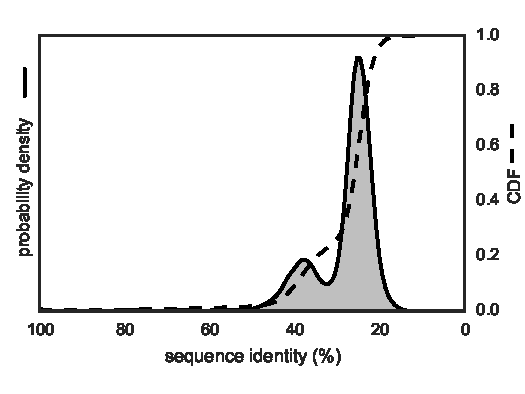
\includegraphics[width=1.0\columnwidth]{seqid_dist/seqid_dist.pdf}

    \caption{{\bf Sequence identity distribution for human TK models.}
    Distribution of sequence identities for all \num{373513} models generated for the human tyrosine kinases.
    Sequence identities are calculated from pairwise target-template alignments.
    The cumulative distribution function is shown by the dashed line.
    The plotted distributions have been smoothed using kernel density estimation.
    % {\color{red}[JDC: Font size too small.]}
    }
  \label{figure:sequence-identity-distribution}
\end{figure}

%%%%%%%%%%%%%%%%%%%%%%%%%%%%%%%%%%%%%%%%%%%%%%%%%%%%%%%%%%%%%%%%%%%%%%%%%%%%%%%%%%%%%%%%%%%%%%%%%%%%%
% FIGURE: RMSD distribution by sequence identity
%%%%%%%%%%%%%%%%%%%%%%%%%%%%%%%%%%%%%%%%%%%%%%%%%%%%%%%%%%%%%%%%%%%%%%%%%%%%%%%%%%%%%%%%%%%%%%%%%%%%%

\begin{figure}[tb]
    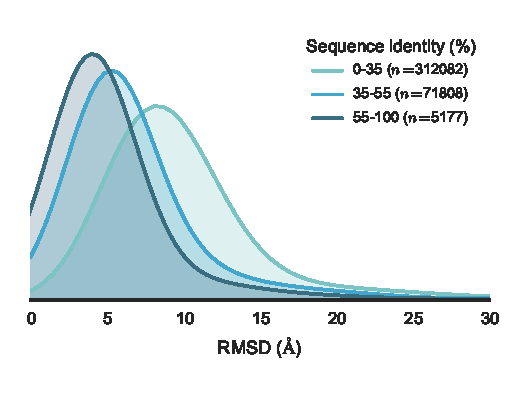
\includegraphics[width=1.0\columnwidth]{rmsddist/rmsddist2.pdf}

    \caption{{\bf RMSD distribution by sequence identity.}
    RMSD distributions for all \num{373513} human TK models, divided into three sequence identity ranges.
    For a given target, model RMSDs are calculated relative to the highest sequence identity model for that target.
    The plotted distributions have been smoothed using kernel density estimation.
    % {\color{red}[JDC: Font size too small.]}
  }
  \label{figure:rmsd-distribution-by-sequence-identity}
\end{figure}

%%%%%%%%%%%%%%%%%%%%%%%%%%%%%%%%%%%%%%%%%%%%%%%%%%%%%%%%%%%%%%%%%%%%%%%%%%%%%%%%%%%%%%%%%%%%%%%%%%%%%
% FIGURE: Superposition of Src and Abl1 sequence identity classes
%%%%%%%%%%%%%%%%%%%%%%%%%%%%%%%%%%%%%%%%%%%%%%%%%%%%%%%%%%%%%%%%%%%%%%%%%%%%%%%%%%%%%%%%%%%%%%%%%%%%%

\begin{figure}[tb]
    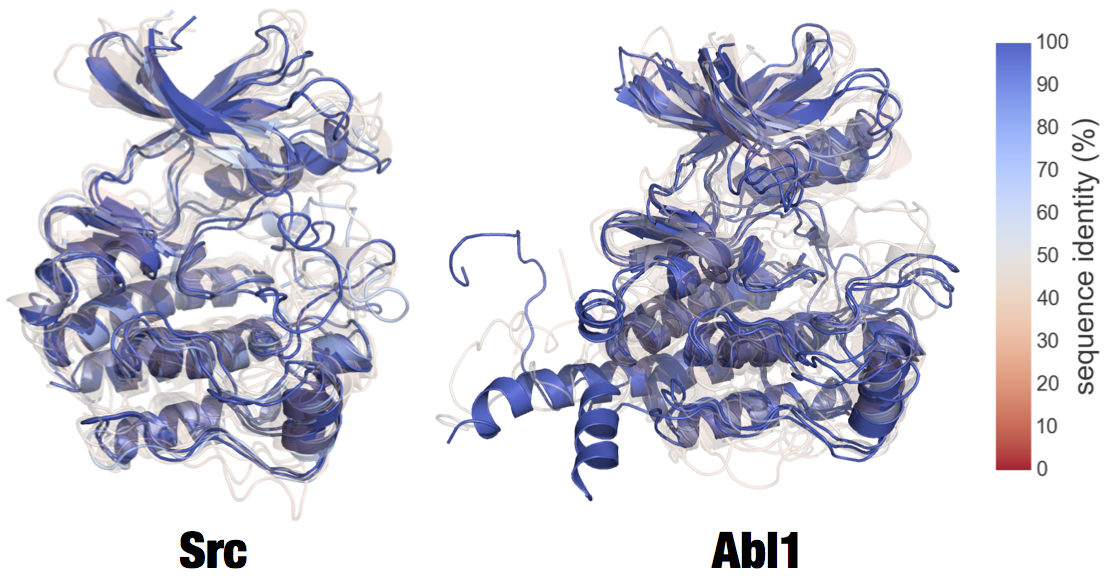
\includegraphics[width=1.0\columnwidth]{superposition-src_abl/superposed-seqid_classes-clustered-one_fig}
    
    \caption{{\bf Superposition of clustered models of Src and Abl1.}
    Superposed renderings of nine models each for Src and Abl1, 
    {\color{red}[JDC: Src and Abl, or Src and Abl1? The description should match the captions above.]}
    {\color{blue}[DLP: Addressed. Using Abl1, as this is the HGNC recommended symbol.]}
    giving some indication the diversity of conformations generated by Ensembler.
    The models for each target were divided into three sequence identity ranges (as in Fig. \ref{figure:rmsd-distribution-by-sequence-identity}), and RMSD-based $k$-medoids clustering was performed to select three clusters from each.
    The models shown are the centroids of each cluster.
    Models are colored and given transparency based on their sequence identity, so that high sequence identity models are blue and opaque, while lower sequence identity models are transparent and red.
    % {\color{red}[JDC: Font size too small.]}
  }
  \label{figure:superposition}
\end{figure}

%%%%%%%%%%%%%%%%%%%%%%%%%%%%%%%%%%%%%%%%%%%%%%%%%%%%%%%%%%%%%%%%%%%%%%%%%%%%%%%%%%%%%%%%%%%%%%%%%%%%%
% FIGURE: Reference structures for Src
%%%%%%%%%%%%%%%%%%%%%%%%%%%%%%%%%%%%%%%%%%%%%%%%%%%%%%%%%%%%%%%%%%%%%%%%%%%%%%%%%%%%%%%%%%%%%%%%%%%%%

\begin{figure}[tb]
    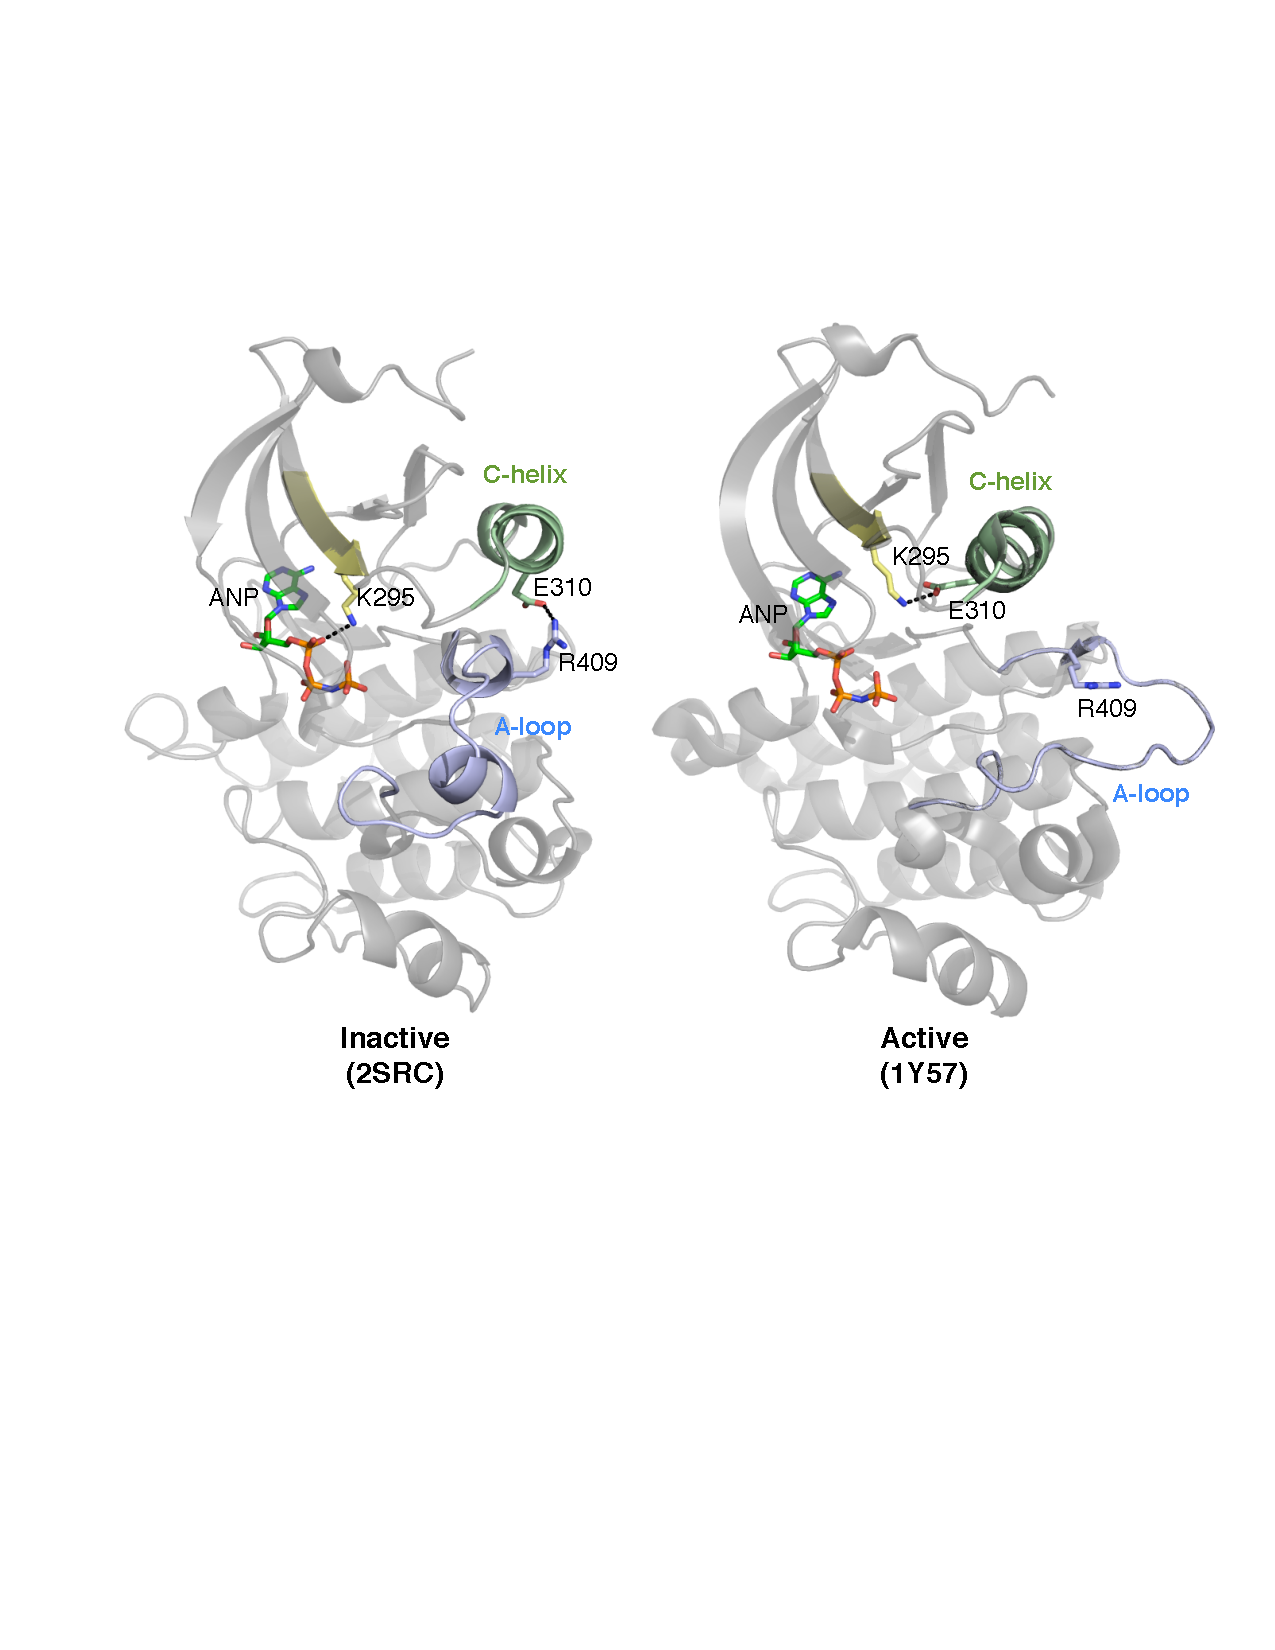
\includegraphics[width=1.0\textwidth]{residue_pair_distances/src/src_ref_structures}
    
    \caption{{\bf Two structures of Src, indicating certain residues involved in activation.}
    In the inactive state, E310 forms a salt bridge with R409.
    During activation, the $\alpha$C-helix (green) moves and rotates, orienting E310 towards the ATP-binding site and allowing it to instead form a salt bridge with K295.
    This positions K295 in the appropriate position for catalysis.
  }
  \label{figure:src-ref-structures}
\end{figure}

%%%%%%%%%%%%%%%%%%%%%%%%%%%%%%%%%%%%%%%%%%%%%%%%%%%%%%%%%%%%%%%%%%%%%%%%%%%%%%%%%%%%%%%%%%%%%%%%%%%%%
% FIGURE: Residue pair distance plots
%%%%%%%%%%%%%%%%%%%%%%%%%%%%%%%%%%%%%%%%%%%%%%%%%%%%%%%%%%%%%%%%%%%%%%%%%%%%%%%%%%%%%%%%%%%%%%%%%%%%%

\begin{figure*}

    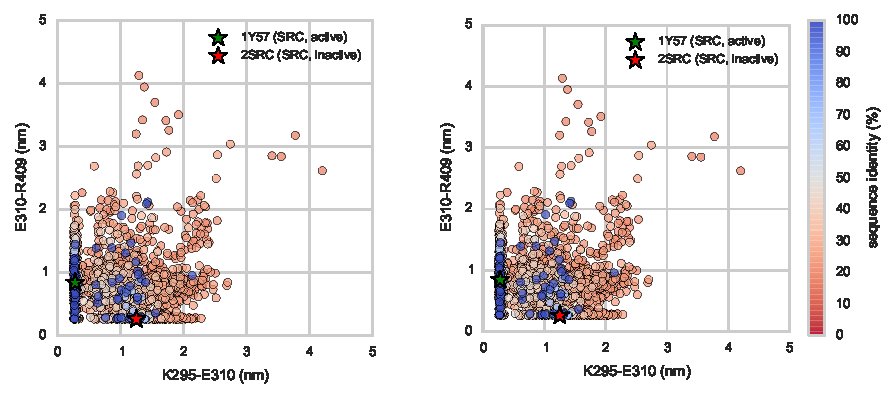
\includegraphics[width=1.0\columnwidth]{residue_pair_distances/src_abl_combined/distances.pdf}

    \caption{{\bf Src and Abl1 models projected onto the distances between two conserved residue pairs, colored by sequence identity.}
    Two Src structures (PDB entries 1Y57 [CITE] and 2SRC [CITE]) are projected onto the plots for reference, representing active and inactive states respectively.
    These structures and the residue pairs analyzed here are depicted in Fig.~\ref{figure:src-ref-structures}.
    Distances are measured between the center of masses of the three terminal sidechain heavy atoms of each residue.
    The atom names for these atoms, according to the PDB coordinate files for both reference structures, are---Lys: NZ, CD, CE (ethylamine); Glu: OE1, CD, OE2 (carboxylate); Arg: NH1, CZ, NH2 (part of guanidine).
    % {\color{red}[JDC: Font size too small if single-column, so I made this double-column. Not sure if that's what you want.]}
    % {\color{red}[JDC: Fill in rest of caption.]}
    }
  \label{figure:pair-distances}
\end{figure*}

%%%%%%%%%%%%%%%%%%%%%%%%%%%%%%%%%%%%%%%%%%%%%%%%%%%%%%%%%%%%%%%%%%%%%%%%%%%%%%%%%%%%%%%%%%%%%%%%%%%%%
% DISCUSSION
%%%%%%%%%%%%%%%%%%%%%%%%%%%%%%%%%%%%%%%%%%%%%%%%%%%%%%%%%%%%%%%%%%%%%%%%%%%%%%%%%%%%%%%%%%%%%%%%%%%%%
\section{Availability and Future Directions}
\label{section:availability}

The latest release of {\bf Ensembler} can be installed via the {\tt conda} package manager for Python~\cite{conda}.
\shellcmd{conda install -c https://conda.binstar.org/omnia ensembler}
Up to date instructions can be found at \url{https://github.com/choderalab/ensembler}.
This will install all dependencies except for Modeller and Rosetta, which are not available through the {\tt conda} package manager, and thus must be installed separately by the user.
The latest source can be downloaded from the above GitHub repository, which also contains instructions for building and installing the code.

% Limitations:
% counterions
% PTMs
% long loops

{\color{red}[JDC: In the Discussion, let's be sure to talk about the limitations and what could be improved or added in the future.  For example, we don't yet handle counterions (e.g. structural Zn$^{2+}$), prosthetic groups (e.g.~heme), or cofactors (e.g.~ATP) yet.  We don't handle post-translational modifications either (such as phosphorylation, methylation, glycosylation, etc.).  It's a good idea to suggest that this is an important first step toward enabling superfamily- and genomics-scale modeling, but there's a lot of work yet to be done.]}

% TODO future directions
% TODO what's on the Ensembler 2 roadmap?
% TODO MCCE?

% TODO CITE: Shan Shaw Proton-dependent switch Abl1 PNAS 2009

%%%%%%%%%%%%%%%%%%%%%%%%%%%%%%%%%%%%%%%%%%%%%%%%%%%%%%%%%%%%%%%%%%%%%%%%%%%%%%%%%%%%%%%%%%%%%%%%%%%%%
% ACKNOWLEDGMENTS
%%%%%%%%%%%%%%%%%%%%%%%%%%%%%%%%%%%%%%%%%%%%%%%%%%%%%%%%%%%%%%%%%%%%%%%%%%%%%%%%%%%%%%%%%%%%%%%%%%%%%
\section{Acknowledgments}
\label{section:acknowledgments}

The authors are grateful to Kyle A.~Beauchamp (MSKCC), Robert McGibbon (Stanford), Arien S. Rustenburg (MSKCC) for many excellent software engineering suggestions.
The authors thank Sonya M.~Hanson (MSKCC), Nicholas M.~Levinson (?), Markus A.~Seeliger (Stony Brook), Diwakar Shukla (Stanford), and Avner Schlessinger (Mount Sinai) for helpful scientific feedback on modeling kinases.
The authors are grateful to Benjamin Webb and Andrej Sali (UCSF) for help with the MODELLER package, Peter Eastman and Vijay Pande (Stanford) for assistance with OpenMM, and Marilyn Gunner (CCNY) for assistance with MCCE2.
DLP and this work was supported in part by the generous support of a Louis V.~Gerstner Young Investigator Award.

%%%%%%%%%%%%%%%%%%%%%%%%%%%%%%%%%%%%%%%%%%%%%%%%%%%%%%%%%%%%%%%%%%%%%%%%%%%%%%%%%%%%%%%%%%%%%%%%%%%%%%
% BIBLIOGRAPHY
%%%%%%%%%%%%%%%%%%%%%%%%%%%%%%%%%%%%%%%%%%%%%%%%%%%%%%%%%%%%%%%%%%%%%%%%%%%%%%%%%%%%%%%%%%%%%%%%%%%%%%

%\bibliographystyle{prsty} 
\bibliography{ms.bib}

%%%%%%%%%%%%%%%%%%%%%%%%%%%%%%%%%%%%%%%%%%%%%%%%%%%%%%%%%%%%%%%%%%%%%%%%%%%%%%%%%%%%%%%%%%%%%%%%%%%%%%
% APPENDICES
%%%%%%%%%%%%%%%%%%%%%%%%%%%%%%%%%%%%%%%%%%%%%%%%%%%%%%%%%%%%%%%%%%%%%%%%%%%%%%%%%%%%%%%%%%%%%%%%%%%%%%

\onecolumngrid
\newpage
\appendix
\setcounter{figure}{0}

\renewcommand{\thesection}{\arabic{section}}
\section{Sequences and residue numbering schemes for Src and Abl1}
\label{si:residue-numbering-schemes}

Kinase catalytic domains are highlighted in red, and the conserved residues analyzed in the main text (Figs.~\ref{figure:src-ref-structures} and~\ref{figure:pair-distances}) are highlighted with yellow background.

\subsubsection*{Human Abl1 sequence}

\begin{alltt}
1     MLEICLKLVG CKSKKGLSSS SSCYLEEALQ RPVASDFEPQ GLSEAARWNS KENLLAGPSE    60
61    NDPNLFVALY DFVASGDNTL SITKGEKLRV LGYNHNGEWC EAQTKNGQGW VPSNYITPVN   120
121   SLEKHSWYHG PVSRNAAEYL LSSGINGSFL VRESESSPGQ RSISLRYEGR VYHYRINTAS   180
181   DGKLYVSSES RFNTLAELVH HHSTVADGLI TTLHYPAPKR NKPTVYGVSP NYDKWEMERT   240
241   D{\color{red}ITMKHKLGG GQYGEVYEGV WKKYSLTVAV {\setlength{\fboxsep}{0pt}\colorbox{yellow}{K}}TLKEDTMEV EEFLK{\setlength{\fboxsep}{0pt}\colorbox{yellow}{E}}AAVM KEIKHPNLVQ}   300
301   {\color{red}LLGVCTREPP FYIITEFMTY GNLLDYLREC NRQEVNAVVL LYMATQISSA MEYLEKKNFI}   360
361   {\color{red}HRDLAARNCL VGENHLVKVA DFGLS{\setlength{\fboxsep}{0pt}\colorbox{yellow}{R}}LMTG DTYTAHAGAK FPIKWTAPES LAYNKFSIKS}   420
421   {\color{red}DVWAFGVLLW EIATYGMSPY PGIDLSQVYE LLEKDYRMER PEGCPEKVYE LMRACWQWNP}   480
481   {\color{red}SDRPSFAEIH QAF}ETMFQES SISDEVEKEL GKQGVRGAVS TLLQAPELPT KTRTSRRAAE   540
541   HRDTTDVPEM PHSKGQGESD PLDHEPAVSP LLPRKERGPP EGGLNEDERL LPKDKKTNLF   600
601   SALIKKKKKT APTPPKRSSS FREMDGQPER RGAGEEEGRD ISNGALAFTP LDTADPAKSP   660
661   KPSNGAGVPN GALRESGGSG FRSPHLWKKS STLTSSRLAT GEEEGGGSSS KRFLRSCSAS   720
721   CVPHGAKDTE WRSVTLPRDL QSTGRQFDSS TFGGHKSEKP ALPRKRAGEN RSDQVTRGTV   780
781   TPPPRLVKKN EEAADEVFKD IMESSPGSSP PNLTPKPLRR QVTVAPASGL PHKEEAGKGS   840
841   ALGTPAAAEP VTPTSKAGSG APGGTSKGPA EESRVRRHKH SSESPGRDKG KLSRLKPAPP   900
901   PPPAASAGKA GGKPSQSPSQ EAAGEAVLGA KTKATSLVDA VNSDAAKPSQ PGEGLKKPVL   960
961   PATPKPQSAK PSGTPISPAP VPSTLPSASS ALAGDQPSST AFIPLISTRV SLRKTRQPPE  1020
1021  RIASGAITKG VVLDSTEALC LAISRNSEQM ASHSAVLEAG KNLYTFCVSY VDSIQQMRNK  1080
1081  FAFREAINKL ENNLRELQIC PATAGSGPAA TQDFSKLLSS VKEISDIVQR             1130
\end{alltt}

\subsubsection*{Sequences for human and chicken Src, aligned using Clustal Omega}

\begin{alltt}
SRC_HUMAN   1     MGSNKSKPKD ASQRRRSLEP AENVHGAGGG AFPASQTPSK PASADGHRGP SAAFAPAAAE    60
SRC_CHICK   1     MGSSKSKPKD PSQRRRSLEP PDSTH---HG GFPASQTPNK TAAPDTHRTP SRSFGTVATE    57
                  ***.******  *********  :..*    * .*******.*  *: * ** * * :*. .*:*  
SRC_HUMAN   61    PKLFGGFNSS DTVTSPQRAG PLAGGVTTFV ALYDYESRTE TDLSFKKGER LQIVNNTEGD   120
SRC_CHICK   58    PKLFGGFNTS DTVTSPQRAG ALAGGVTTFV ALYDYESRTE TDLSFKKGER LQIVNNTEGD   117
                  ********:* **********  ********* ********** ********** **********  
SRC_HUMAN   121   WWLAHSLSTG QTGYIPSNYV APSDSIQAEE WYFGKITRRE SERLLLNAEN PRGTFLVRES   180
SRC_CHICK   118   WWLAHSLTTG QTGYIPSNYV APSDSIQAEE WYFGKITRRE SERLLLNPEN PRGTFLVRES   177
                  *******:** ********** ********** ********** ******* ** **********  
SRC_HUMAN   181   ETTKGAYCLS VSDFDNAKGL NVKHYKIRKL DSGGFYITSR TQFNSLQQLV AYYSKHADGL   240
SRC_CHICK   178   ETTKGAYCLS VSDFDNAKGL NVKHYKIRKL DSGGFYITSR TQFSSLQQLV AYYSKHADGL   237
                  ********** ********** ********** ********** ***.****** **********  
SRC_HUMAN   241   CHRLTTVCPT SKPQTQGLAK DAWEIPRES{\color{red}L RLEVKLGQGC FGEVWMGTWN GTTRVAI{\setlength{\fboxsep}{0pt}\colorbox{yellow}{K}}TL}   300
SRC_CHICK   238   CHRLTNVCPT SKPQTQGLAK DAWEIPRES{\color{red}L RLEVKLGQGC FGEVWMGTWN GTTRVAI{\setlength{\fboxsep}{0pt}\colorbox{yellow}{K}}TL}   297
                  *****.**** ********** ********** ********** ********** **********  
SRC_HUMAN   301   {\color{red}KPGTMSPEAF LQ{\setlength{\fboxsep}{0pt}\colorbox{yellow}{E}}AQVMKKL RHEKLVQLYA VVSEEPIYIV TEYMSKGSLL DFLKGETGKY}   360
SRC_CHICK   298   {\color{red}KPGTMSPEAF LQ{\setlength{\fboxsep}{0pt}\colorbox{yellow}{E}}AQVMKKL RHEKLVQLYA VVSEEPIYIV TEYMSKGSLL DFLKGEMGKY}   357
                  ********** ********** ********** ********** ********** ****** ***  
SRC_HUMAN   361   {\color{red}LRLPQLVDMA AQIASGMAYV ERMNYVHRDL RAANILVGEN LVCKVADFGL A{\setlength{\fboxsep}{0pt}\colorbox{yellow}{R}}LIEDNEYT}   420
SRC_CHICK   358   {\color{red}LRLPQLVDMA AQIASGMAYV ERMNYVHRDL RAANILVGEN LVCKVADFGL A{\setlength{\fboxsep}{0pt}\colorbox{yellow}{R}}LIEDNEYT}   417
                  ********** ********** ********** ********** ********** **********  
SRC_HUMAN   421   {\color{red}ARQGAKFPIK WTAPEAALYG RFTIKSDVWS FGILLTELTT KGRVPYPGMV NREVLDQVER}   480
SRC_CHICK   418   {\color{red}ARQGAKFPIK WTAPEAALYG RFTIKSDVWS FGILLTELTT KGRVPYPGMV NREVLDQVER}   477
                  ********** ********** ********** ********** ********** **********  
SRC_HUMAN   481   {\color{red}GYRMPCPPEC PESLHDLMCQ CWRKEPEERP TFEYLQAFLE DYF}TSTEPQY QPGENL       536
SRC_CHICK   478   {\color{red}GYRMPCPPEC PESLHDLMCQ CWRKDPEERP TFEYLQAFLE DYF}TSTEPQY QPGENL       533
                  ********** ********** ****:***** ********** ********** ******
\end{alltt}

\section{Figures}

\begin{figure*}[h]
    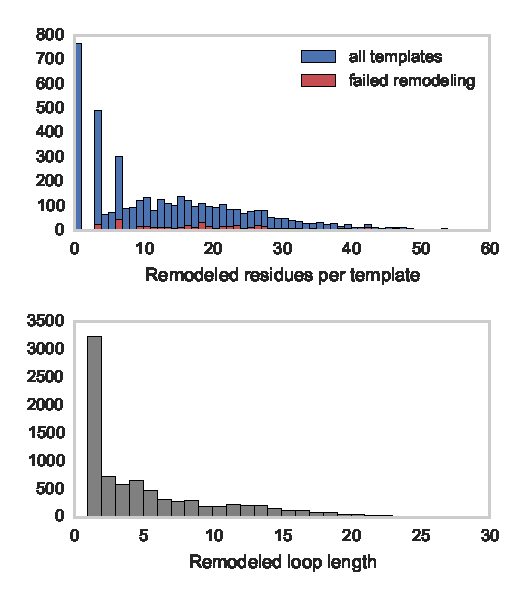
\includegraphics[width=0.5\textwidth]{loopmodel_analysis/nmissing_resis_distributions.pdf}
    \caption{{\bf Distributions for the number of missing residues for templates for which remodeling (with the {\tt loopmodel} command) was either successful or unsuccessful.}
    The plotted distributions are smoothed using kernel density estimation, and the raw data points are shown as a rug plot.
    }
    \label{si:loopmodel-nmissing-residues}
\end{figure*}

\end{document}
